\documentclass[10pt,twocolumn]{article}  % 10pt font, two-column format

% Math formula support
\usepackage{amsmath}
% Graphics support
\usepackage{graphicx}
% Set graphics path
\graphicspath{{Picic/}}
% Bibliography support
\usepackage{natbib}
\usepackage{titlesec}
\usepackage{titling}
\usepackage{geometry}
\usepackage{algorithm}
\usepackage{algorithmic}
% Hyperlink support
\usepackage{hyperref}
\usepackage{placeins}
\usepackage{times}                      % Times New Roman font
\usepackage{mathptmx}                   % Times font for math symbols
\usepackage{xcolor}
\usepackage{etoolbox}
\usepackage{caption}
\definecolor{myPink}{RGB}{255,105,180}  % Define pink color
\date{}  % Remove date
\hypersetup{
    colorlinks=true,       % 启用链接颜色
    linkcolor=blue,        % 内部链接颜色
    citecolor=blue,        % 引用文献颜色
    urlcolor=myPink        % URL 颜色
}
\geometry{
    a4paper,            % A4 纸张
    textwidth=17.46cm,  % 文本区域宽度
    textheight=22.54cm, % 文本区域高度
    columnsep=0.8cm,    % 栏间距
    top=2.54cm,         % 首页标题距顶部距离
    bottom=3.5cm,       % 下边距
    left=1.9cm,         % 左边距
    right=1.9cm,        % 右边距
    headheight=0.5cm,   % 页眉高度
    headsep=0.2cm,      % 页眉与正文的间距
    footskip=0.8cm      % 页脚与正文的间距
}

% Set document title
\title{Momentum Contrast for Unsupervised Visual Representation Learning}
% Set author information
\author{Kaiming He \quad Haoqi Fan \quad Yuxin Wu \quad Saining Xie \quad Ross Girshick \\
\\
Facebook AI Research (FAIR) \\
Code: \href{https://github.com/facebookresearch/moco}{\color{myPink}https://github.com/facebookresearch/moco}
}

% 调整标题上方的空白

% \renewcommand{\abstractname}{\normalfont\bfseries\large Abstract1243} % 12pt Times 粗体,居中
% \titleformat{\abstract}{\normalfont\bfseries\large}{\centering}{0em}{}
% \titlespacing{\abstract}{0pt}{0pt}{0pt} % 移除摘要标题的默认间距
\newcommand{\mylinebreak}{\linebreak\hspace*{1em}}
\titleformat{\section}{\normalfont\Large\bfseries}{\thesection.}{0.2em}{}
\titlespacing*{\section}{0pt}{0.5em}{0.5em} % 根据需要调整负值的大小

\makeatletter
\renewenvironment{abstract}{%
    \begin{center}%
        \normalfont\bfseries\large Abstract% 保持标题样式
    \end{center}%
    \begin{minipage}{0.5\textwidth}% 约束行宽
    \fontsize{10pt}{12pt}\selectfont% 强制字号
    \noindent% 取消首行缩进
    \itshape% 斜体正文
}
{%
    \end{minipage}%
}
\makeatother

\begin{document}
\maketitle

% Abstract section
\begin{abstract}
    \fontsize{10pt}{12pt}\selectfont % 10pt 字体,单倍行距
    \noindent % 完全对齐
    \itshape \hspace{1em} We present Momentum Contrast (MoCo) for unsuper-
    vised visual representation learning. From a perspective on
    contrastive learning \cite{29_hadsell2006dimensionality} as dictionary look-up, we build
    a dynamic dictionary with a queue and a moving-averaged
    encoder. This enables building a large and consistent dic-
    tionary on-the-fly that facilitates contrastive unsupervised
    learning. MoCo provides competitive results under the
    common linear protocol on ImageNet classification. More
    importantly, the representations learned by MoCo transfer
    well to downstream tasks. MoCo can outperform its super-
    vised pre-training counterpart in 7 detection/segmentation
    tasks on PASCAL VOC, COCO, and other datasets, some-
    times surpassing it by large margins. This suggests that
    the gap between unsupervised and supervised representa-
    tion learning has been largely closed in many vision tasks.
\end{abstract}

% Main body
\section{Introduction}
\hspace{1em} Unsupervised representation learning is highly success-
ful in natural language processing, e.g., as shown by GPT
\cite{50_radford2018improving, 51_radford2019language} and BERT \cite{12_devlin2019bert}. But supervised pre-training is still
dominant in computer vision, where unsupervised meth-
ods generally lag behind. The reason may stem from dif-
ferences in their respective signal spaces. Language tasks
have discrete signal spaces (words, sub-word units, etc.)
for building tokenized dictionaries, on which unsupervised
learning can be based. Computer vision, in contrast, further
concerns dictionary building \cite{54_sivic2003video, 9_coates2011importance, 5_chatfield2011devil}, as the raw signal is
in a continuous, high-dimensional space and is not struc-
tured for human communication (e.g., unlike words).
Several recent studies \cite{61_wu2018unsupervised, 46_oord2018representation, 36_hjelm2019learning, 66_zhuang2019local, 35_henaff2019data, 56_tian2019contrastive, 2_bachman2019learning}
present promising results on unsupervised visual representation
learning using approaches related to the contrastive loss
\cite{29_hadsell2006dimensionality}. Though driven by various motivations, these methods
can be thought of as building dynamic dictionaries. The
“keys” (tokens) in the dictionary are sampled from data
(e.g., images or patches) and are represented by an encoder
network. Unsupervised learning trains encoders to perform
dictionary look-up: an encoded “query” should be similar
to its matching key and dissimilar to others. Learning is
formulated as minimizing a contrastive loss \cite{29_hadsell2006dimensionality}.

\begin{figure}[t]
    \centering
    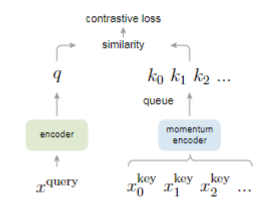
\includegraphics[width=0.75\linewidth]{Pic/figure1.png} % 图片路径和宽度
    \caption{Momentum Contrast (MoCo) trains a visual represen-
    tation encoder by matching an encoded query q to a dictionary
    of encoded keys using a contrastive loss. The dictionary keys
    {k0, k1, k2, ...} are defined on-the-fly by a set of data samples.
    The dictionary is built as a queue, with the current mini-batch en-
    queued and the oldest mini-batch dequeued, decoupling it from
    the mini-batch size. The keys are encoded by a slowly progressing
    encoder, driven by a momentum update with the query encoder.
    This method enables a large and consistent dictionary for learning
    visual representations.} % 图片标题
    \label{fig:Figure 1} % 图片标签
    \vspace{-1em} % 压缩标题下方空白
\end{figure}
% \vspace{2.5em} % 图片下方添加间距

From this perspective, we hypothesize that it is desirable
to build dictionaries that are: (i) large and (ii) consistent
as they evolve during training. Intuitively, a larger dictio-
nary may better sample the underlying continuous, high-
dimensional visual space, while the keys in the dictionary
should be represented by the same or similar encoder so that
their comparisons to the query are consistent. However, ex-
isting methods that use contrastive losses can be limited in
one of these two aspects (discussed later in context).
\mylinebreak We present Momentum Contrast (MoCo) as a way of
building large and consistent dictionaries for unsupervised
learning with a contrastive loss (Figure 1). We maintain the
dictionary as a queue of data samples: the encoded repre-
sentations of the current mini-batch are enqueued, and the
oldest are dequeued. The queue decouples the dictionary
size from the mini-batch size, allowing it to be large. More-
over, as the dictionary keys come from the preceding sev-
eral mini-batches, a slowly progressing key encoder, imple-
mented as a momentum-based moving average of the query
encoder, is proposed to maintain consistency.
MoCo is a mechanism for building dynamic dictionar-
ies for contrastive learning, and can be used with various
pretext tasks. In this paper, we follow a simple instance
discrimination task \cite{61_wu2018unsupervised, 63_ye2019unsupervised, 2_bachman2019learning}:
a query matches a key if
they are encoded views (e.g., different crops) of the same
image. Using this pretext task, MoCo shows competitive
results under the common protocol of linear classification
in the ImageNet dataset \cite{11_deng2009imagenet}.
A main purpose of unsupervised learning is to pre-train
representations (i.e., features) that can be transferred to
downstream tasks by fine-tuning. We show that in 7 down-
stream tasks related to detection or segmentation, MoCo
unsupervised pre-training can surpass its ImageNet super-
vised counterpart, in some cases by nontrivial margins. In
these experiments, we explore MoCo pre-trained on Ima-
geNet or on a one-billion Instagram image set, demonstrat-
ing that MoCo can work well in a more real-world, billion-
image scale, and relatively uncurated scenario. These re-
sults show that MoCo largely closes the gap between un-
supervised and supervised representation learning in many
computer vision tasks, and can serve as an alternative to Im-
ageNet supervised pre-training in several applications.

\section{Related Work}
\hspace{1em} Unsupervised/self-supervised1 learning methods gener-
ally involve two aspects: pretext tasks and loss functions.
The term “pretext” implies that the task being solved is not
of genuine interest, but is solved only for the true purpose
of learning a good data representation. Loss functions can
often be investigated independently of pretext tasks. MoCo
focuses on the loss function aspect. Next we discuss related
studies with respect to these two aspects.
Loss functions. A common way of defining a loss function
is to measure the difference between a model's prediction
and a fixed target, such as reconstructing the input pixels
(e.g., auto-encoders) by L1 or L2 losses, or classifying the
input into pre-defined categories (e.g., eight positions \cite{13_doersch2015unsupervised},
color bins \cite{64_zhang2016colorful}) by cross-entropy or margin-based losses.
Other alternatives, as described next, are also possible.
Contrastive losses \cite{29_hadsell2006dimensionality} measure the similarities of sam-
ple pairs in a representation space. Instead of matching an
input to a fixed target, in contrastive loss formulations the
target can vary on-the-fly during training and can be defined
in terms of the data representation computed by a network
\cite{29_hadsell2006dimensionality}. Contrastive learning is at the core of several recent
works on unsupervised learning \cite{61_wu2018unsupervised, 46_oord2018representation, 36_hjelm2019learning, 66_zhuang2019local, 35_henaff2019data, 56_tian2019contrastive, 2_bachman2019learning},
which we elaborate on later in context (Sec. 3.1).
Adversarial losses \cite{24_goodfellow2014generative} measure the difference between
probability distributions. It is a widely successful technique
for unsupervised data generation. Adversarial methods for
representation learning are explored in \cite{15_donahue2017adversarial, 16_donahue2019large}. There are
relations (see \cite{24_goodfellow2014generative}) between generative adversarial networks
and noise-contrastive estimation (NCE) \cite{28_gutmann2010noise}.
Pretext tasks. A wide range of pretext tasks have been pro-
posed. Examples include recovering the input under some
corruption, e.g., denoising auto-encoders \cite{58_vincent2008denoising}, context auto-
encoders \cite{48_pathak2016context}, or cross-channel auto-encoders (coloriza-
tion) \cite{64_zhang2016colorful, 65_zhang2017splitbrain}. Some pretext tasks form pseudo-labels by,
e.g., transformations of a single (“exemplar”) image \cite{17_dosovitskiy2014discriminative},
patch orderings \cite{13_doersch2015unsupervised, 45_noroozi2016unsupervised}, tracking \cite{59_wang2015unsupervised} or segmenting ob-
jects \cite{47_pathak2017learning} in videos, or clustering features \cite{3_caron2018deep, 4_caron2019unsupervised}.
Contrastive learning vs. pretext tasks. Various pretext
tasks can be based on some form of contrastive loss func-
tions. The instance discrimination method \cite{61_wu2018unsupervised} is related
to the exemplar-based task \cite{17_dosovitskiy2014discriminative} and NCE \cite{28_gutmann2010noise}. The pretext
task in contrastive predictive coding (CPC) \cite{46_oord2018representation} is a form
of context auto-encoding \cite{48_pathak2016context}, and in contrastive multiview
coding (CMC) \cite{56_tian2019contrastive} it is related to colorization \cite{64_zhang2016colorful}.

\section{Method}
\subsection{Contrastive Learning as Dictionary Look-up}
\hspace{1em} Contrastive learning \cite{29_hadsell2006dimensionality}, and its recent developments,
can be thought of as training an encoder for a dictionary
look-up task, as described next.
Consider an encoded query q and a set of encoded sam-
ples {k0, k1, k2, ...} that are the keys of a dictionary. As-
sume that there is a single key (denoted as k+) in the dic-
tionary that q matches. A contrastive loss \cite{29_hadsell2006dimensionality} is a function
whose value is low when q is similar to its positive key k+
and dissimilar to all other keys (considered negative keys
for q). With similarity measured by dot product, a form of
a contrastive loss function, called InfoNCE \cite{46_oord2018representation}, is consid-
ered in this paper:

%公式1
\begin{equation}
    L(q, k+) = -\log\frac{\exp(q^T k^+)}{\sum_{i=0}^K \exp(q^T k_i^+)}
    \label{eq:equation1}
\end{equation}

where $\tau$ is a temperature hyper-parameter per \cite{61_wu2018unsupervised}. The sum
is over one positive and K negative samples. Intuitively,
this loss is the log loss of a (K+1)-way softmax-based clas-
sifier that tries to classify q as k+. Contrastive loss functions
can also be based on other forms \cite{29_hadsell2006dimensionality, 59_wang2015unsupervised, 61_wu2018unsupervised, 36_hjelm2019learning}, such as
margin-based losses and variants of NCE losses.
The contrastive loss serves as an unsupervised objective
function for training the encoder networks that represent the
queries and keys \cite{29_hadsell2006dimensionality}. In general, the query representation
is q = fq(xq ) where fq is an encoder network and xq is a
query sample (likewise, k = fk(xk)). Their instantiations
depend on the specific pretext task. The input xq and xk can
be images \cite{29_hadsell2006dimensionality, 61_wu2018unsupervised, 63_ye2019unsupervised}, patches \cite{46_oord2018representation}, or context consisting a
set of patches \cite{46_oord2018representation}. The networks fq and fk can be identical
\cite{29_hadsell2006dimensionality, 59_wang2015unsupervised, 63_ye2019unsupervised}, partially shared \cite{46_oord2018representation, 36_hjelm2019learning, 2_bachman2019learning}, or different \cite{56_tian2019contrastive}.

\begin{figure*}[htbp]
    \centering
    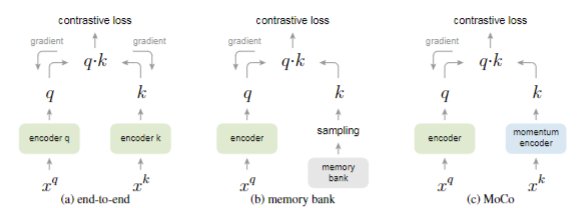
\includegraphics[width=0.8\linewidth]{Pic/figure2.png} % 图片路径和宽度
    \caption{Conceptual comparison of three contrastive loss mechanisms (empirical comparisons are in Figure 3 and Table 3). Here we
    illustrate one pair of query and key. The three mechanisms differ in how the keys are maintained and how the key encoder is updated.
    (a): The encoders for computing the query and key representations are updated end-to-end by back-propagation (the two encoders can
    be different). (b): The key representations are sampled from a memory bank \cite{61_wu2018unsupervised}. (c): MoCo encodes the new keys on-the-fly by a
    momentum-updated encoder, and maintains a queue (not illustrated in this figure) of keys.} % 图片标题
    \label{fig:Figure 2} % 图片标签
\end{figure*}

\subsection{Momentum Contrast}
\hspace{1em} From the above perspective, contrastive learning is a way
of building a discrete dictionary on high-dimensional con-
tinuous inputs such as images. The dictionary is dynamic in
the sense that the keys are randomly sampled, and that the
key encoder evolves during training. Our hypothesis is that
good features can be learned by a large dictionary that cov-
ers a rich set of negative samples, while the encoder for the
dictionary keys is kept as consistent as possible despite its
evolution. Based on this motivation, we present Momentum
Contrast as described next.
Dictionary as a queue. At the core of our approach is
maintaining the dictionary as a queue of data samples. This
allows us to reuse the encoded keys from the immediate pre-
ceding mini-batches. The introduction of a queue decouples
the dictionary size from the mini-batch size. Our dictionary
size can be much larger than a typical mini-batch size, and
can be flexibly and independently set as a hyper-parameter.
The samples in the dictionary are progressively replaced.
The current mini-batch is enqueued to the dictionary, and
the oldest mini-batch in the queue is removed. The dictio-
nary always represents a sampled subset of all data, while
the extra computation of maintaining this dictionary is man-
ageable. Moreover, removing the oldest mini-batch can be
beneficial, because its encoded keys are the most outdated
and thus the least consistent with the newest ones.
Momentum update. Using a queue can make the dictio-
nary large, but it also makes it intractable to update the key
encoder by back-propagation (the gradient should propa-
gate to all samples in the queue). A na\"{\i}ve solution is to
copy the key encoder fk from the query encoder fq, ignor-
ing this gradient. But this solution yields poor results in
experiments (Sec. 4.1). We hypothesize that such failure
is caused by the rapidly changing encoder that reduces the
key representations' consistency. We propose a momentum
update to address this issue.
Formally, denoting the parameters of $f_k$ as $\theta_k$ and those
of $f_q$ as $\theta_q$, we update $\theta_k$ by:

%公式2
\begin{equation}
    \theta_k = m \theta_k + (1-m) \theta_q
    \label{eq:equation2}
\end{equation}

Here m $\epsilon$ [0, 1) is a momentum coefficient. Only the pa-
rameters $\theta_q$ are updated by back-propagation. The momen-
tum update in Eqn.(2) makes $\theta_k$ evolve more smoothly than
$\theta_q$. As a result, though the keys in the queue are encoded
by different encoders (in different mini-batches), the dif-
ference among these encoders can be made small. In ex-
periments, a relatively large momentum (e.g., m = 0.999,
our default) works much better than a smaller value (e.g.,
m = 0.9), suggesting that a slowly evolving key encoder is
a core to making use of a queue.
Relations to previous mechanisms. MoCo is a general
mechanism for using contrastive losses. We compare it with
two existing general mechanisms in Figure 2. They exhibit
different properties on the dictionary size and consistency.
The end-to-end update by back-propagation is a natural
mechanism (e.g., \cite{29_hadsell2006dimensionality, 46_oord2018representation, 36_hjelm2019learning, 63_ye2019unsupervised, 2_bachman2019learning, 35_henaff2019data}, Figure 2a). It uses
samples in the current mini-batch as the dictionary, so the
keys are consistently encoded (by the same set of encoder
parameters). But the dictionary size is coupled with the
mini-batch size, limited by the GPU memory size. It is also
challenged by large mini-batch optimization \cite{25_goyal2017accurate}. Some re-
cent methods \cite{46_oord2018representation, 36_hjelm2019learning, 2_bachman2019learning} are based on pretext tasks driven by
local positions, where the dictionary size can be made larger
by multiple positions. But these pretext tasks may require
special network designs such as patchifying the input \cite{46_oord2018representation}
or customizing the receptive field size \cite{2_bachman2019learning}, which may com-
plicate the transfer of these networks to downstream tasks.
Another mechanism is the memory bank approach pro-
posed by \cite{61_wu2018unsupervised} (Figure 2b). A memory bank consists of the
representations of all samples in the

%伪代码
% \FloatBarrier
% \clearpage % 强制分页
\begin{algorithm}[t!]
    \caption{Pseudocode of MoCo in a PyTorch-like style.}
    \label{alg:al1}
    % \mdseries
    \begin{algorithmic}[0]
    \fontseries{l}\selectfont
    % \renewcommand{\algorithmicindent}{0em}
    \renewcommand{\algorithmiccomment}[1]{}
    \STATE \# $f_q$, $f_k$: encoder networks for query and key
    \STATE \# queue: dictionary as a queue of K keys (CxK)
    \STATE \# m: momentum
    \STATE \# t: temperature
    \STATE
    \STATE \texttt{f\_k}.params = \texttt{f\_q}.params  \#  initialize
    \STATE for x in loader: \# load a minibatch x with N samples
    \STATE \hspace{2em}\texttt{x\_q} = aug(x) \# a randomly augmented version
    \STATE \hspace{2em}\texttt{x\_k} = aug(x) \# another randomly augmented version
    \STATE
    \STATE \hspace{2em}q = \texttt{f\_q}.forward(\texttt{x\_q}) \# queries: NxC
    \STATE \hspace{2em}k = \texttt{f\_k}.forward(\texttt{x\_k}) \# keys: NxC
    \STATE \hspace{2em}k = k.detach() \# no gradient to keys
    \STATE
    \STATE \hspace{2em}\# positive logits: Nx1
    \STATE \hspace{2em}\texttt{l\_pos} = bmm(q.view(N,1,C), k.view(N,C,1))
    \STATE
    \STATE \hspace{2em}\# negative logits: NxK
    \STATE \hspace{2em}\texttt{l\_neg} = mm(q.view(N,C), queue.view(C,K))
    \STATE
    \STATE \hspace{2em}\# logits: Nx(1+K)
    \STATE \hspace{2em}logits = cat([\texttt{l\_pos}, \texttt{l\_neg}], dim=1)
    \STATE
    \STATE \hspace{2em}\# contrastive loss, Eqn.(1)
    \STATE \hspace{2em}labels = zeros(N) \# positives are the 0-th
    \STATE \hspace{2em}loss = CrossEntropyLoss(logits/t, labels)
    \STATE
    \STATE \hspace{2em}\# SGD update: query network
    \STATE \hspace{2em}loss.backward()
    \STATE \hspace{2em}update(\texttt{f\_q}.params)
    \STATE
    \STATE \hspace{2em}\# momentum update: key network
    \STATE \hspace{2em}\texttt{f\_k}.params = m*\texttt{f\_k}.params+(1-m)*\texttt{f\_q}.params
    \STATE
    \STATE \hspace{2em}\# update dictionary
    \STATE \hspace{2em}enqueue(queue, k) \# enqueue the current minibatch
    \STATE \hspace{2em}dequeue(queue) \# dequeue the earliest minibatch
    \STATE
    \end{algorithmic}
\end{algorithm}

% \vskip 2\baselineskip
%     {\footnotesize\hangindent=2em\hangafter=1
%     \textbf{bmm: batch matrix multiplication; mm: matrix multiplication; cat: concatenation.}}
% \end{algorithm}

% \smallskip
\vspace{-3em} % 调整间距
\textbf{\small bmm: batch matrix multiplication; mm: matrix multiplication; cat: concatenation.}



dataset. The dictionary
for each mini-batch is randomly sampled from the memory
bank with no back-propagation, so it can support a large
dictionary size. However, the representation of a sample in 
the memory bank was updated when it was last seen, so the
sampled keys are essentially about the encoders at multiple
different steps all over the past epoch and thus are less con-
sistent. A momentum update is adopted on the memory
bank in \cite{61_wu2018unsupervised}. Its momentum update is on the representa-
tions of the same sample, not the encoder. This momentum
update is irrelevant to our method, because MoCo does not
keep track of every sample. Moreover, our method is more
memory-efficient and can be trained on billion-scale data,
which can be intractable for a memory bank.
Sec. 4 empirically compares these three mechanisms.

\subsection{Pretext Task}
Contrastive learning can drive a variety of pretext tasks.
As the focus of this paper is not on designing a new pretext
task, we use a simple one mainly following the instance
discrimination task in \cite{61_wu2018unsupervised},
to which some recent works \cite{63_ye2019unsupervised, 2_bachman2019learning} are related.
Following \cite{61_wu2018unsupervised}, we consider a query and a key as a pos-
itive pair if they originate from the same image, and other-
wise as a negative sample pair. Following \cite{63_ye2019unsupervised, 2_bachman2019learning}, we take
two random “views” of the same image under random data
augmentation to form a positive pair. The queries and keys
are respectively encoded by their encoders, $f_q$ and $f_k$. The
encoder can be any convolutional neural network \cite{39_lecun1989backpropagation}.
Algorithm 1 provides the pseudo-code of MoCo for this
pretext task. For the current mini-batch, we encode the
queries and their corresponding keys, which form the posi-
tive sample pairs. The negative samples are from the queue.
Technical details. We adopt a ResNet \cite{39_lecun1989backpropagation} as the encoder,
whose last fully-connected layer (after global average pool-
ing) has a fixed-dimensional output (128-D \cite{61_wu2018unsupervised}). This out-
put vector is normalized by its L2-norm \cite{61_wu2018unsupervised}. This is the
representation of the query or key. The temperature $\tau$ in
Eqn.(1) is set as 0.07 \cite{61_wu2018unsupervised}. The data augmentation setting
follows \cite{61_wu2018unsupervised}: a 224$\times$224-pixel crop is taken from a ran-
domly resized image, and then undergoes random color jit-
tering, random horizontal flip, and random grayscale con-
version, all available in PyTorch's torchvision package.
Shuffling BN. Our encoders fq and fk both have Batch
Normalization (BN) \cite{37_ioffe2015batch} as in the standard ResNet \cite{33_he2016deep}. In
experiments, we found that using BN prevents the model
from learning good representations, as similarly reported
in \cite{35_henaff2019data} (which avoids using BN). The model appears to
“cheat” the pretext task and easily finds a low-loss solu-
tion. This is possibly because the intra-batch communica-
tion among samples (caused by BN) leaks information.
We resolve this problem by shuffling BN. We train with
multiple GPUs and perform BN on the samples indepen-
dently for each GPU (as done in common practice). For the
key encoder fk, we shuffle the sample order in the current
mini-batch before distributing it among GPUs (and shuffle
back after encoding); the sample order of the mini-batch
for the query encoder fq is not altered. This ensures the
batch statistics used to compute a query and its positive key
come from two different subsets. This effectively tackles
the cheating issue and allows training to benefit from BN.
We use shuffled BN in both our method and its end-to-
end ablation counterpart (Figure 2a). It is irrelevant to the
memory bank counterpart (Figure 2b), which does not suf-
fer from this issue because the positive keys are from differ-
ent mini-batches in the past.

\section{Experiments}
\hspace{1em} We study unsupervised training performed in:
ImageNet-1M (IN-1M): This is the ImageNet \cite{11_deng2009imagenet} train-
ing set that has $\sim$1.28 million images in 1000 classes (often
called ImageNet-1K; we count the image number instead,
as classes are not exploited by unsupervised learning). This
dataset is well-balanced in its class distribution, and its im-
ages generally contain iconic view of objects.
Instagram-1B (IG-1B): Following \cite{44_mahajan2018exploring}, this is a dataset
of $\sim$1 billion (940M) public images from Instagram. The
images are from $\sim$1500 hashtags \cite{44_mahajan2018exploring} that are related to the
ImageNet categories. This dataset is relatively uncurated
comparing to IN-1M, and has a long-tailed, unbalanced
distribution of real-world data. This dataset contains both
iconic objects and scene-level images.
Training. We use SGD as our optimizer. The SGD weight
decay is 0.0001 and the SGD momentum is 0.9. For IN-1M,
we use a mini-batch size of 256 (N in Algorithm 1) in 8
GPUs, and an initial learning rate of 0.03. We train for 200
epochs with the learning rate multiplied by 0.1 at 120 and
160 epochs \cite{61_wu2018unsupervised}, taking $\sim$53 hours training ResNet-50. For
IG-1B, we use a mini-batch size of 1024 in 64 GPUs, and
a learning rate of 0.12 which is exponentially decayed by
0.9$\times $ after every 62.5k iterations (64M images). We train
for 1.25M iterations ($\sim$1.4 epochs of IG-1B), taking $\sim$6 days
for ResNet-50.


\subsection{Linear Classification Protocol}
We first verify our method by linear classification on
frozen features, following a common protocol. In this sub-
section we perform unsupervised pre-training on IN-1M.
Then we freeze the features and train a supervised linear
classifier (a fully-connected layer followed by softmax). We
train this classifier on the global average pooling features of
a ResNet, for 100 epochs. We report 1-crop, top-1 classifi-
cation accuracy on the ImageNet validation set.
For this classifier, we perform a grid search and find the
optimal initial learning rate is 30 and weight decay is 0
(similarly reported in \cite{56_tian2019contrastive}). These hyper-parameters per-
form consistently well for all ablation entries presented in
this subsection. These hyper-parameter values imply that
the feature distributions (e.g., magnitudes) can be substan-
tially different from those of ImageNet supervised training,
an issue we will revisit in Sec. 4.2.
Ablation: contrastive loss mechanisms. We compare the
three mechanisms that are illustrated in Figure 2. To focus
on the effect of contrastive loss mechanisms, we implement
all of them in the same pretext task as described in Sec. 3.3.
We also use the same form of InfoNCE as the contrastive
loss function, Eqn.(1). As such, the comparison is solely on
the three mechanisms.
The results are in Figure 3. Overall, all three mecha-
nisms benefit from a larger K. A similar trend has been
observed in \cite{61_wu2018unsupervised, 56_tian2019contrastive} under the memory bank mechanism,
while here we show that this trend is more general and can
be seen in all mechanisms. These results support our moti-
vation of building a large dictionary.
The end-to-end mechanism performs similarly to MoCo
when K is small. However, the dictionary size is limited
by the mini-batch size due to the end-to-end requirement.
Here the largest mini-batch a high-end machine (8 Volta
32GB GPUs) can afford is 1024. More essentially, large
mini-batch training is an open problem \cite{25_goyal2017accurate}: we found it
necessary to use the linear learning rate scaling rule \cite{25_goyal2017accurate}
here, without which the accuracy drops (by $\sim$2% with a
1024 mini-batch). But optimizing with a larger mini-batch
is harder \cite{25_goyal2017accurate}, and it is questionable whether the trend can
be extrapolated into a larger K even if memory is sufficient.

\begin{figure}[htbp]
    \centering
    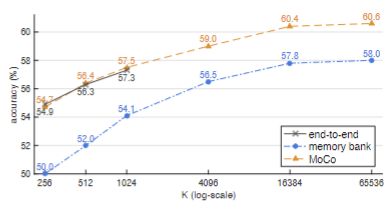
\includegraphics[width=0.8\linewidth]{Pic/figure3.png} % 图片路径和宽度
    \caption{ Comparison of three contrastive loss mechanisms un-
    der the ImageNet linear classification protocol. We adopt the same
    pretext task (Sec. 3.3) and only vary the contrastive loss mecha-
    nism (Figure 2). The number of negatives is K in memory bank
    and MoCo, and is K--1 in end-to-end (offset by one because the
    positive key is in the same mini-batch). The network is ResNet-50.} % 图片标题
    \label{fig:Figure 3} % 图片标签
\end{figure}

The memory bank \cite{61_wu2018unsupervised} mechanism can support a larger
dictionary size. But it is 2.6% worse than MoCo. This is
inline with our hypothesis: the keys in the memory bank
are from very different encoders all over the past epoch and
they are not consistent. Note the memory bank result of
58.0% reflects our improved implementation of \cite{61_wu2018unsupervised}.2
Ablation: momentum. The table below shows ResNet-50
accuracy with different MoCo momentum values (m in
Eqn.(2)) used in pre-training (K = 4096 here) :

\begin{table}[htbp]
    \centering
    \begin{tabular}{c|c} % 定义两列,无外边框
        momentum m & 0 0.9 0.99 0.999 0.9999 \\ 
        \hline % 水平线
        accuracy (\%) & fail 55.2 57.8 59.0 5809 \\ 
    \end{tabular}
    \label{tab:tab} % 表格标签
\end{table}

It performs reasonably well when m is in 0.99 $\sim $ 0.9999,
showing that a slowly progressing (i.e., relatively large mo-
mentum) key encoder is beneficial. When m is too small
(e.g., 0.9), the accuracy drops considerably; at the extreme
of no momentum (m is 0), the training loss oscillates and
fails to converge. These results support our motivation of
building a consistent dictionary.
Comparison with previous results. Previous unsuper-
vised learning methods can differ substantially in model
sizes. For a fair and comprehensive comparison, we report
accuracy vs. \#parameters3 trade-offs. Besides ResNet-50
(R50) \cite{33_he2016deep}, we also report its variants that are 2$\times $ and 4$\times $
wider (more channels), following \cite{38_kolesnikov2019revisiting}.4 We set K = 65536
and m = 0.999. Table 1 is the comparison.
MoCo with R50 performs competitively and achieves
60.6% accuracy, better than all competitors of similar
model sizes ($\sim $24M). MoCo benefits from larger models and
achieves 68.6% accuracy with R50w4×.
Notably, we achieve competitive results using a standard
ResNet-50 and require no specific architecture designs, e.g.,

% table1
\begin{figure}[t!]
    \centering
    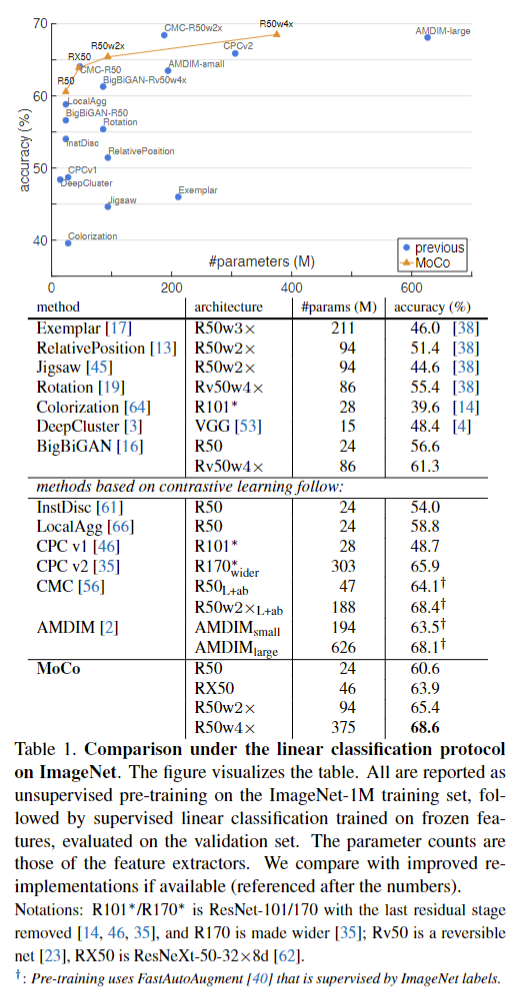
\includegraphics[width=1\linewidth]{Pic/table1.png} % 图片路径和宽度
    \captionsetup{labelformat=empty}
    \caption{Table 1. Comparison under the linear classification protocol
    on ImageNet. The figure visualizes the table. All are reported as
    unsupervised pre-training on the ImageNet-1M training set, fol-
    lowed by supervised linear classification trained on frozen fea-
    tures, evaluated on the validation set. The parameter counts are
    those of the feature extractors. We compare with improved re-
    implementations if available (referenced after the numbers).
    Notations: R101$\ast $/R170$\ast $ is ResNet-101/170 with the last residual stage
    removed \cite{14_doersch2017multi, 46_oord2018representation, 35_henaff2019data},
    and R170 is made wider \cite{35_henaff2019data}; Rv50 is a reversible
    net \cite{23_gomez2017reversible}, RX50 is ResNeXt-50-32$\times $8d \cite{62_xie2017residual}.
    $\dagger$: Pre-training uses FastAutoAugment \cite{40_lim2019fast} that is supervised by ImageNet labels.} % 图片标题
    \label{fig:Table 1} % 图片标签
    \vspace{-1em}
\end{figure}

patchified inputs \cite{46_oord2018representation, 35_henaff2019data}, carefully tailored receptive fields
\cite{2_bachman2019learning}, or combining two networks \cite{56_tian2019contrastive}. By using an architec-
ture that is not customized for the pretext task, it is easier to
transfer features to a variety of visual tasks and make com-
parisons, studied in the next subsection.
This paper's focus is on a mechanism for general con-
trastive learning; we do not explore orthogonal factors (such
as specific pretext tasks) that may further improve accuracy.
As an example, “MoCo v2” \cite{8_chen2020improved}, an extension of a prelim-
inary version of this manuscript, achieves 71.1% accuracy
with R50 (up from 60.6%), given small changes on the data
augmentation and output projection head \cite{7_chen2020simple}. We believe
that this additional result shows the generality and robust-
ness of the MoCo framework.

% table2
\begin{figure}[t!]
    \centering
    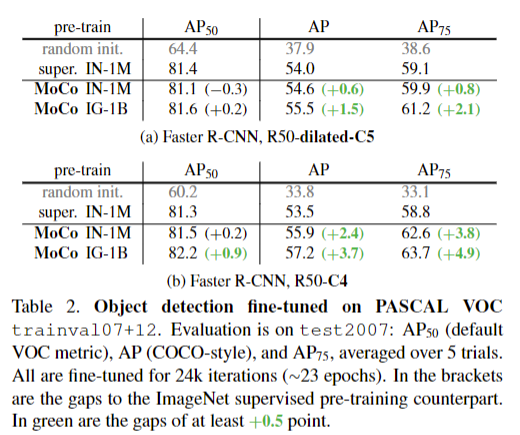
\includegraphics[width=1\linewidth]{Pic/table2.png} % 图片路径和宽度
    \captionsetup{labelformat=empty}
    \caption{Table 2. Object detection fine-tuned on PASCAL VOC
    trainval07+12. Evaluation is on test2007: AP50 (default
    VOC metric), AP (COCO-style), and AP75, averaged over 5 trials.
    All are fine-tuned for 24k iterations ($\sim $23 epochs). In the brackets
    are the gaps to the ImageNet supervised pre-training counterpart.
    In green are the gaps of at least +0.5 point.} % 图片标题
    \label{fig:Table 2} % 图片标签
    \vspace{-1em}
\end{figure}
% table3
\begin{figure}[t!]
    \centering
    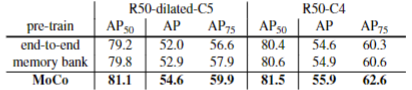
\includegraphics[width=1\linewidth]{Pic/table3.png} % 图片路径和宽度
    \captionsetup{labelformat=empty}
    \caption{Table 3. Comparison of three contrastive loss mechanisms on
    PASCAL VOC object detection, fine-tuned on trainval07+12
    and evaluated on test2007 (averages over 5 trials). All models
    are implemented by us (Figure 3), pre-trained on IN-1M, and fine-
    tuned using the same settings as in Table 2.} % 图片标题
    \label{fig:Table 3} % 图片标签
    \vspace{-1em}
\end{figure}

\subsection{Transferring Features}
A main goal of unsupervised learning is to learn features
that are transferrable. ImageNet supervised pre-training is
most influential when serving as the initialization for fine-
tuning in downstream tasks (e.g., \cite{21_girshick2014rich,20_girshick2015fast, 43_long2015fully, 52_ren2015faster}). Next
we compare MoCo with ImageNet supervised pre-training,
transferred to various tasks including PASCAL VOC \cite{18_everingham2010pascal},
COCO \cite{42_lin2014microsoft}, etc. As prerequisites, we discuss two important
issues involved \cite{31_he2019rethinking}: normalization and schedules.
Normalization. As noted in Sec. 4.1, features produced by
unsupervised pre-training can have different distributions
compared with ImageNet supervised pre-training. But a
system for a downstream task often has hyper-parameters
(e.g., learning rates) selected for supervised pre-training. To
relieve this problem, we adopt feature normalization during
fine-tuning: we fine-tune with BN that is trained (and syn-
chronized across GPUs \cite{49_peng2018megdet}), instead of freezing

% table4
\FloatBarrier
\begin{figure*}[t!]
    \centering
    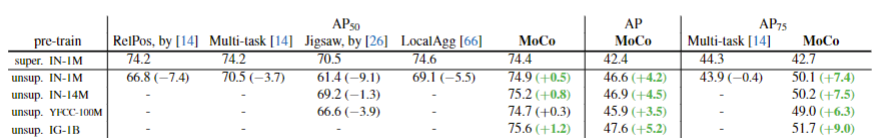
\includegraphics[width=1\linewidth]{Pic/table4.png} % 图片路径和宽度
    \captionsetup{labelformat=empty} % 新增此行
    \caption{Table 4. Comparison with previous methods on object detection fine-tuned on PASCAL VOC trainval2007. Evaluation is on
    test2007. The ImageNet supervised counterparts are from the respective papers, and are reported as having the same structure as the
    respective unsupervised pre-training counterparts. All entries are based on the C4 backbone. The models in [14] are R101 v2 [34], and
    others are R50. The RelPos (relative position) [13] result is the best single-task case in the Multi-task paper [14]. The Jigsaw [45] result is
    from the ResNet-based implementation in [26]. Our results are with 9k-iteration fine-tuning, averaged over 5 trials. In the brackets are the
    gaps to the ImageNet supervised pre-training counterpart. In green are the gaps of at least +0.5 point.} % 图片标题
    \label{fig:Table 4} % 图片标签
\end{figure*}

it by an affine layer \cite{33_he2016deep}. We also use BN in the newly initialized
layers (e.g., FPN \cite{41_lin2017feature}), which helps calibrate magnitudes.
We perform normalization when fine-tuning supervised
and unsupervised pre-training models. MoCo uses the same
hyper-parameters as the ImageNet supervised counterpart.
Schedules. If the fine-tuning schedule is long enough,
training detectors from random initialization can be strong
baselines, and can match the ImageNet supervised counter-
part on COCO \cite{31_he2019rethinking}. Our goal is to investigate transferabil-ity
of features, so our experiments are on controlled sched-
ules, e.g., the 1$\times $ ($\sim $12 epochs) or 2$\times $ schedules \cite{22_girshick2018detectron} for
COCO, in contrast to 6$\times $$\sim $9$\times $ in \cite{31_he2019rethinking}. On smaller datasets
like VOC, training longer may not catch up \cite{31_he2019rethinking}.
Nonetheless, in our fine-tuning, MoCo uses the same
schedule as the ImageNet supervised counterpart, and ran-
dom initialization results are provided as references.
Put together, our fine-tuning uses the same setting as the
supervised pre-training counterpart. This may place MoCo
at a disadvantage. Even so, MoCo is competitive. Doing so
also makes it feasible to present comparisons on multiple
datasets/tasks, without extra hyper-parameter search.
\subsubsection{PASCAL VOC Object Detection}
Setup. The detector is Faster R-CNN \cite{52_ren2015faster} with a backbone
of R50-dilated-C5 or R50-C4 \cite{32_he2017mask} (details in appendix),
with BN tuned, implemented in \cite{60_wu2019detectron2}. We fine-tune all lay-
ers end-to-end. The image scale is [480, 800] pixels during
training and 800 at inference. The same setup is used for all
entries, including the supervised pre-training baseline. We
evaluate the default VOC metric of AP50 (i.e., IoU threshold
is 50%) and the more stringent metrics of COCO-style AP
and AP75. Evaluation is on the VOC test2007 set.
Ablation: backbones. Table 2 shows the results fine-tuned
on trainval07+12 ($\sim $16.5k images). For R50-dilated-
C5 (Table 2a), MoCo pre-trained on IN-1M is comparable
to the supervised pre-training counterpart, and MoCo pre-
trained on IG-1B surpasses it. For R50-C4 (Table 2b),
MoCo with IN-1M or IG-1B is better than the supervised
counterpart: up to +0.9 AP50, +3.7 AP, and +4.9 AP75.
Interestingly, the transferring accuracy depends on the
detector structure. For the C4 backbone, by default used
in existing ResNet-based results \cite{14_doersch2017multi, 61_wu2018unsupervised, 26_goyal2019scaling, 66_zhuang2019local}, the ad-
vantage of unsupervised pre-training is larger. The relation
between pre-training vs. detector structures has been veiled
in the past, and should be a factor under consideration.
Ablation: contrastive loss mechanisms. We point out that
these results are partially because we establish solid detec-
tion baselines for contrastive learning. To pin-point the gain
that is solely contributed by using the MoCo mechanism
in contrastive learning, we fine-tune the models pre-trained
with the end-to-end or memory bank mechanism, both im-
plemented by us (i.e., the best ones in Figure 3), using the
same fine-tuning setting as MoCo.
These competitors perform decently (Table 3). Their AP
and AP75 with the C4 backbone are also higher than the
ImageNet supervised counterpart's, c.f . Table 2b, but other
metrics are lower. They are worse than MoCo in all metrics.
This shows the benefits of MoCo. In addition, how to train
these competitors in larger-scale data is an open question,
and they may not benefit from IG-1B.
Comparison with previous results. Following the com-
petitors, we fine-tune on trainval2007 ($\sim $5k images)
using the C4 backbone. The comparison is in Table 4.
For the AP50 metric, no previous method can catch
up with its respective supervised pre-training counterpart.
MoCo pre-trained on any of IN-1M, IN-14M (full Ima-
geNet), YFCC-100M \cite{55_thomee2016yfcc100m}, and IG-1B can outperform the
supervised baseline. Large gains are seen in the more strin-
gent metrics: up to +5.2 AP and +9.0 AP75. These gains are
larger than the gains seen in trainval07+12 (Table 2b).

\subsubsection{COCO Object Detection and Segmentation}
Setup. The model is Mask R-CNN \cite{32_he2017mask} with the FPN \cite{41_lin2017feature}
or C4 backbone, with BN tuned, implemented in \cite{60_wu2019detectron2}. The
image scale is in [640, 800] pixels during training and is 800
at inference. We fine-tune all layers end-to-end. We fine-
tune on the train2017 set ($\sim $118k images) and evaluate
on val2017. The schedule is the default 1$\times $ or 2$\times $ in


\FloatBarrier
\begin{figure*}[h!]
    \centering
    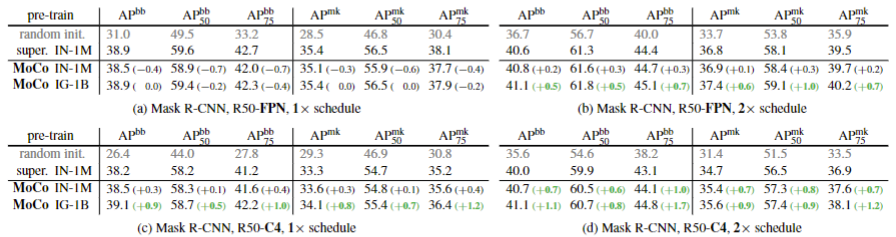
\includegraphics[width=0.8\linewidth]{Pic/table5.png} % 图片路径和宽度
    \captionsetup{labelformat=empty}
    \caption{Table 5. Object detection and instance segmentation fine-tuned on COCO: bounding-box AP (APbb) and mask AP (APmk) evaluated
    on val2017. In the brackets are the gaps to the ImageNet supervised pre-training counterpart. In green are the gaps of at least +0.5 point.} % 图片标题
    \label{fig:Table 5} % 图片标签
\end{figure*}


\FloatBarrier
\begin{figure}[h!]
    \centering
    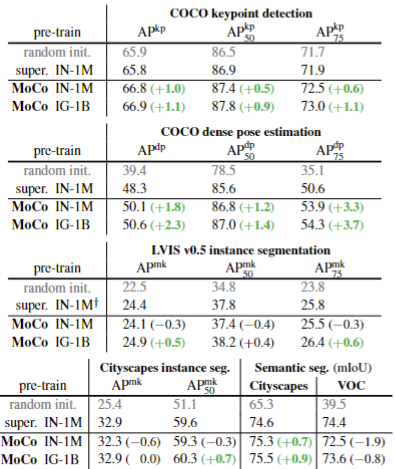
\includegraphics[width=1\linewidth]{Pic/table6.png} % 图片路径和宽度
    \captionsetup{labelformat=empty}
    \caption{Table 6. MoCo vs. ImageNet supervised pre-training, fine-
    tuned on various tasks. For each task, the same architecture and
    schedule are used for all entries (see appendix). In the brackets are
    the gaps to the ImageNet supervised pre-training counterpart. In
    green are the gaps of at least +0.5 point.
    $\dagger$:: this entry is with BN frozen, which improves results; see main text.} % 图片标题
    \label{fig:Table 6} % 图片标签
\end{figure}

\cite{22_girshick2018detectron}.
Results. Table 5 shows the results on COCO with the FPN
(Table 5a, b) and C4 (Table 5c, d) backbones. With the
1$\times $ schedule, all models (including the ImageNet super-
vised counterparts) are heavily under-trained, as indicated
by the $\sim $2 points gaps to the 2$\times $ schedule cases. With the
2$\times $ schedule, MoCo is better than its ImageNet supervised
counterpart in all metrics in both backbones.

\subsubsection{More Downstream Tasks}
Table 6 shows more downstream tasks (implementation de-
tails in appendix). Overall, MoCo performs competitively

with ImageNet supervised pre-training:
COCO keypoint detection: supervised pre-training has
no clear advantage over random initialization, whereas
MoCo outperforms in all metrics.
COCO dense pose estimation \cite{1_guler2018densepose}: MoCo substantially
outperforms supervised pre-training, e.g., by 3.7 points in
APdp
75, in this highly localization-sensitive task.
LVIS v0.5 instance segmentation \cite{27_gupta2019lvis}: this task has
$\sim $1000 long-tailed distributed categories. Specifically in
LVIS for the ImageNet supervised baseline, we find fine-
tuning with frozen BN (24.4 APmk) is better than tunable
BN (details in appendix). So we compare MoCo with the
better supervised pre-training variant in this task. MoCo
with IG-1B surpasses it in all metrics.
Cityscapes instance segmentation \cite{10_cordts2016cityscapes}: MoCo with IG-1B
is on par with its supervised pre-training counterpart in
APmk, and is higher in APmk
50 .
Semantic segmentation: On Cityscapes \cite{10_cordts2016cityscapes}, MoCo out-
performs its supervised pre-training counterpart by up to 0.9
point. But on VOC semantic segmentation, MoCo is worse
by at least 0.8 point, a negative case we have observed.
Summary. In sum, MoCo can outperform its ImageNet
supervised pre-training counterpart in 7 detection or seg-
mentation tasks.5 Besides, MoCo is on par on Cityscapes
instance segmentation, and lags behind on VOC semantic
segmentation; we show another comparable case on iNatu-
ralist \cite{57_vanhorn2018inaturalist} in appendix. Overall, MoCo has largely closed
the gap between unsupervised and supervised representa-
tion learning in multiple vision tasks.
Remarkably, in all these tasks, MoCo pre-trained on
IG-1B is consistently better than MoCo pre-trained on
IN-1M. This shows that MoCo can perform well on this
large-scale, relatively uncurated dataset. This represents a
scenario towards real-world unsupervised learning.

\section{Discussion and Conclusion}
\hspace{1em} Our method has shown positive results of unsupervised
learning in a variety of computer vision tasks and datasets.
A few open questions are worth discussing. MoCo's im-
provement from IN-1M to IG-1B is consistently noticeable
but relatively small, suggesting that the larger-scale data
may not be fully exploited. We hope an advanced pretext
task will improve this. Beyond the simple instance discrim-
ination task \cite{61_wu2018unsupervised}, it is possible to adopt MoCo for pretext
tasks like masked auto-encoding, e.g., in language \cite{12_devlin2019bert} and
in vision \cite{46_oord2018representation}. We hope MoCo will be useful with other
pretext tasks that involve contrastive learning.

% Bibliography section
\bibliographystyle{plain}
\bibliography{references}


\end{document}